\color{red}

\subsection{Glyph: \glyph{Entity}}
\label{sec:physicalEntity}

\SBGNERLone defines only one glyph for all entities, whether physical entity, such as protein, a nucleic acid, metabolite or functional entity such as a gene. Indeed the exact nature of entities does not impact the rules of interactions within a diagram. The nature of a particular entity may then be clarified using its label and decorations, as will become clear below. 

\begin{glyphDescription}

\glyphSboTerm SBO:0000245 ! entity 

\glyphContainer An entity is represented by a rectangular container with rounded corners, as illustrated in \fig{entity}.

\glyphLabel An \glyph{entity} is identified by a label placed in an unbordered box containing a string of characters.  The characters can be distributed on several lines to improve readability, although this is not mandatory.  The label box must be attached to the center of the container.  The label may spill outside of the container.

\glyphAux An \glyph{entity} can carry state variables that can add information about its state (\sect{stateVariable}).  A state variable is represented by a rectangle capped with two hemi-circles, with the long axis of this  ``capsule'' placed on the border of the \glyph{entity}'s container, as illustrated in \fig{entity}.  The label of the state variable (which can precise the type of characteristic represented by the state variable, residue type, residue number etc.) is written within the state variable's container. Particular \glyph{state variables} are the existence (\sect{existence}) and the location (\sect{location}).

An \glyph{entity} can also carry one or several \glyph{units of information} (\sect{unitInfo}).  The units of information can characterise a domain, such as a binding site.  Particular \glyph{units of information} are available for describing the material type (\sect{material-types-cv}) and the conceptual type (\sect{conceptual-types-cv}) of a macromolecule.  The center of the bounding box of a \glyph{unit of information} is located on the mid-line of the border of the macromolecule.

\end{glyphDescription}

\begin{figure}[H]
  \centering
  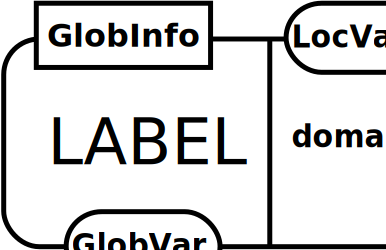
\includegraphics[scale = 0.3]{images/entity}
  \caption{The \ER glyph for \glyph{entity}.}
  \label{fig:macromolecule}
\end{figure}

\normalcolor

% The following is for [X]Emacs users.   Please leave in place.
% Local Variables:
% TeX-master: "../sbgn_ER-level1"
% End:
